% !TEX root = ../thesis-example.tex
%
\chapter{Notations}
\label{ch:notation}

\cleanchapterquote{You know how I adjusted to that problem of\\
the radio in the environment : very much as\\
the primitive people adjusted to the animals\\
which frightened them, and which probably, \\
as you say, were intrusions. They drew pictures\\
of them on their caves and so I simply made \\
a piece using radios. Now, whenever I hear radios\\
--~even a single radio, not just twelve at a time\\
as you must have heard on the beach, at least~--\\
I think : ``Well, they're just playing my piece''.}
{John Cage}{John Cage / Morton Feldman. \\ Radio Happenings, 1966.\\\cite{cage_radio_2015}}
\index[people]{cage@Cage, John!radiohappenings@\textit{Radio Happenings}}
\index[people]{feldman@Feldman, Morton!radiohappenings@\textit{Radio Happenings}}

% \cleanchapterquote{(...) building a musical instrument becomes indistinguishable from designing a music-theoretical framework; the musical instrument is a theory of music (...)}{Thor Magnusson}{Sonic Writing (2019)}

% This article presents “John”, an open-source software designed to help collective free improvisation. It provides generated screen-scores running on distributed, reactive web-browsers. The musicians can then concurrently edit the scores in their own browser. John is used by ONE, a septet playing improvised electro-acoustic music with digital musical instruments (DMI). One of the original features of John is that its design takes care of leaving the
% musician's attention as free as possible.
% Firstly, a quick review of the context of screen-based
% scores will help situate this research in the history of contemporary music notation. Then I will trace back how improvisation sessions led to John's particular “notational perspective”. A brief description of the software will precede a discussion about the various aspects guiding its design.

\vspace*{\fill}

\noindent Dans ce dernier chapitre, j'aborde la question de la notation musicale, dont j'ai déjà évoqué les problèmes qu'elle pose dans le cas des musiques électroacoustiques au chapitre \ref{ch:ephemeral}. En particulier, j'y présente ``John, le semi-conducteur'', un logiciel de partition sur écran développé pour la pratique collective de l'improvisation libre électroacoustique avec l'ensemble \textit{ONE}, et les motivations qui ont conduit à ce développement.\\
\indent Au préalable, je présenterai un état de l'art des partitions sur écran, ainsi qu'un rapide parcours dans l'histoire de la notation musicale à travers ses différents enjeux, en soulignant l'entrelacs qui se tisse entre les pratiques d'analyse, de lutherie, de composition, d'interprétation et d'improvisation, et comment ces différents aspects s'articulent dans les lutheries et les musiques numériques.

\clearpage

%%%%%%%%%%%%%%%%%%%%%%%%%%%%%%%%%%%%%%%%%
\section{Notes sur la partition}

\subsection{La notation comme instrument mnémonique}

\subsubsection{Écrire le passé}

\noindent La notation musicale consiste à transcrire une œuvre musicale sur un support, généralement visuel. Elle est donc, en premier lieu, un moyen de noter \textit{a posteriori} une musique ``passée'' en procédant, par analyse, à l'extraction de caractéristiques saillantes, qui structurent le \textit{continuum} de la performance musicale, et en les représentant de manière symbolique. La notation sert ainsi de moyen mnémonique permettant de garder une trace de la performance musicale et de conserver de manière durable l'image d'un phénomène sonore sinon éphémère.\\
\indent Cette analyse peut s'intéresser aux propriétés du son (telle que sa hauteur, son intensité, etc.) mais également aux gestes et aux matériaux qui le produisent. Ces deux aspects, ont notamment donné lieu à deux systèmes de notation dans la tradition musicale occidentale\footnote{~Notons cependant que cette tendance des sociétés occidentales qui valorisent la culture de l'écrit, associée aux classes sociales plus élevées, davantage que l'oralité, associée aux musiques folkloriques et populaires, n'est pas universelle. La culture hindoue, par exemple, attache une valeur plus importante à l'enseignement oral en ce qui concerne la musique: vouloir noter sur papier ce qu'un maître de tabla enseigne de manière orale y est considéré comme un dilletantisme de la mémoire assez méprisable. Cf. également annexe \ref{appendix:dumeaux}.}, ayant perduré jusqu'à nos jours:
\vspace{-1em}
\begin{itemize}[noitemsep]
	\item la portée musicale, élaborée au \siecle{11}~siècle par Guido d'Arezzo qui modernise la notation neumatique en formalisant la dénomination des notes et la notation solfégique. Ce système constitue une écriture ``phonographique'' du son\footnote{Je reprends ici les termes de notation ``phonographique'' et ``ergographique'' proposés par Eric Maestri dans \cite{maestri_notation_2016}\index[people]{maestri@Maestri, Eric}.}, selon une approche ``esthésique''\footnote{Jean-Jacques Nattiez, dans son analyse sémiologique de la musique \cite{nattiez_musicologie_1987}, distingue un processus ``poïétique'', de création, d'un processus ``esthésique'' de réception de l'œuvre musicale.}, et définie par des caractéristiques du son telle que sa hauteur, son intensité et sa durée, relativement indépendamment des gestes qui concourent à sa production;
	\item la tablature, apparue au début du \siecle{14}~siècle, qui s'attache davantage à la notation ``ergographique'' ou ``poïétique'' du son, en privilégiant la notation des gestes sur un instrument spécifique (en particulier la position des différents doigts sur les instruments à cordes).\footnote{Bien entendu, ces deux approches ne sont pas orthogonales et partagent de nombreux points communs. Leur avantages et inconvénients respectifs les rendent toutefois suffisamment complémentaires, pour que de nombreuses partitions, de guitare en particulier, présentent les deux en parallèle.}
\end{itemize}

\noindent Les techniques d'enregistrement audio inventées à la fin du \siecle{19}~siècle ont permis de conserver les œuvres musicales sans recourir à leur réduction symbolique, mais l'intégration progressive du timbre comme paramètre d'écriture musicale, en particulier dans les musiques électroacoustiques --~qui ne possèdent généralement pas de partition préalable~-- a renouvelé dans le même temps les besoins d'analyse du champ musical ainsi élargi. Des logiciels tels que l'Acousmographe \cite{favreau_lacousmographe_2010} ou EAnalysis \cite{couprie_eanalysis:_2016} sont entièrement dédiés à cette question et de manière plus générale, le domaine interdisciplinaire des \gls{MIR} qui a émergé au tournant du siècle, ainsi que la plus récente conférence \gls{TENOR} continuent d'apporter de nouvelles perspectives sur la notation musicale.

\subsubsection{Écrire pour le futur}

\noindent Si la notation permet de consigner une musique pré-existante, ce processus analytique offre en retour un système symbolique qui possède sa propre logique, et une certaine autonomie. En transposant la \textit{temporalité musicale} en une \textit{spatialité visuelle}\footnote{Voir à ce sujet la notion de ``grammatisation'' présentée au chapitre \ref{ch:gesture}.}, la partition permet d'agencer des symboles musicaux ``hors du temps'' de la performance, et d'écrire ainsi une musique ``pour le futur'' à partir de cette grammaire, utilisée de manière générative. La notation musicale a ainsi permis de créer des œuvres qui auraient difficilement pu être conçues sans ce support visuel\footnote{Un exemple historique notoire est le rondeau ``Ma fin est mon commencement'' (\siecle{14}~siècle) de Guillaume de Machaut\index[people]{machaut@Machaut, Guillaume de!mafinestmoncommencement@\textit{Ma fin est mon commencement}}, dans lequel les deux voix sont rétrogrades l'une à l'autre.}. Ainsi, la partition est généralement considérée comme un document permettant de composer une œuvre musicale et de la transmettre à un instrumentiste en vue de son interprétation. Elle en constitue la forme abstraite par excellence au point d'être souvent assimilée à l'œuvre elle-même dans la tradition musicale occidentale.\\
\indent Cette objetisation de la performance musicale, préalablement immatérielle, éphémère et directe, en une forme tangible, durable et médiatisée a opéré une scission entre les actes de composition et de performance, aux multiples conséquences. Comme le souligne Magnusson dans \cite{magnusson_algorithms_2011}, \iquote{le désir de capturer la musique, la représenter dans le silence des signes écrits et l'invoquer à nouveau par l'interprétation de ces signes} a posé les bases d'une \iquote{industrie de la composition et de l'interprétation de la musique, et surtout, de la technologie et de l'infrastructure nécessaire à l'enregistrement, la distribution et la vente de musique destinée à sa lecture automatique sur machines.}

%extension d'impressions, intension d'expressions
%--------------------------------------------------------------------
\subsection{Des partitions symboliques aux partitions graphiques}

\noindent Le développement des techniques d'écriture dans le système de notation d'Arezzo a conduit à une complexité croissante des œuvres en terme d'orchestration, qui donne naissance aux formes symphoniques de la musique romantique. Cette complexification de la musique s'accompagne également d'un intérêt grandissant pour le timbre, qui mène les partitions a intégrer progressivement des techniques de jeu étendues (\textit{con legno}, \textit{sul ponticello}, etc.) par le biais d'annotations \textit{ad hoc} et de nouveaux symboles pictographiques.\\
\indent Les diverses révolutions technologiques du \siecle{19}~siècle ont bouleversé à la fois les moyens de production et le champ de l'expression musicale. À l'enthousiasme des Futuristes italiens du début du \siecle{20}~siècle --~qui voient dans ces révolutions un moyen de se révolter contre le conservatisme de l'opéra italien, en adoptant l'ensemble des bruits dans le domaine du son musical~--, et ses influences fertiles sur les compositeurs modernes, comme Stravinsky\index[people]{stravinsky@Stravinsky, Igor} ou Varèse\index[people]{varese@Varèse, Edgar}, s'adjoignent des questions plus existentielles de présentation et de représentation musicale.\\
\indent Le ``bruit des machines'', c'est-à-dire la production automatisée et industrialisée des phénomènes audibles (musicaux ou non) a envahi l'espace perceptif, remettant en question la place du son\footnote{On pense notamment à la notion d'écologie sonore qui émerge au milieu du siècle et exemplifiée dans le travail de Raymond Murray Schafer\index[people]{murrayschafer@Murray Schafer, Raymond} \cite{schafer_paysage_1979}.} et de l'œuvre musicale dans la société. Noter le son devient, dans certains cas, impossible dans la mesure où les outils/instruments de production sonore possèdent leur propre logique, possiblement externe à la volonté de l'utilisateur/instrumentiste. Dans les années 1960, le mouvement Fluxus, en particulier, répond à ce problème en accordant une importance primordiale au geste et au processus dans l'écriture de performance\footnote{Un exemple notoire est la pièce ``Imaginary landscape No 4'' de John Cage\index[people]{cage@Cage, John!imaginarylandscapenofour@\textit{Imaginary landscape No 4}}, où l'utilisation de radio rend impossible la description du résultat musical \textit{a priori}, tandis que les gestes de changement de gain et de fréquence sont précisément notés. Pour une étude plus approfondie sur la relation entre partition et action, voire notamment \cite{kojs_notating_2011}.} en inventant de nouvelles représentations pour ces partitions nouvelles (figure \ref{fig:notation:feldman}).\\
%-------------------------- Figure : Morton Feldman ----------------------------------
\begin{figure}[!htbp]
	\captionsetup{format=plain}
	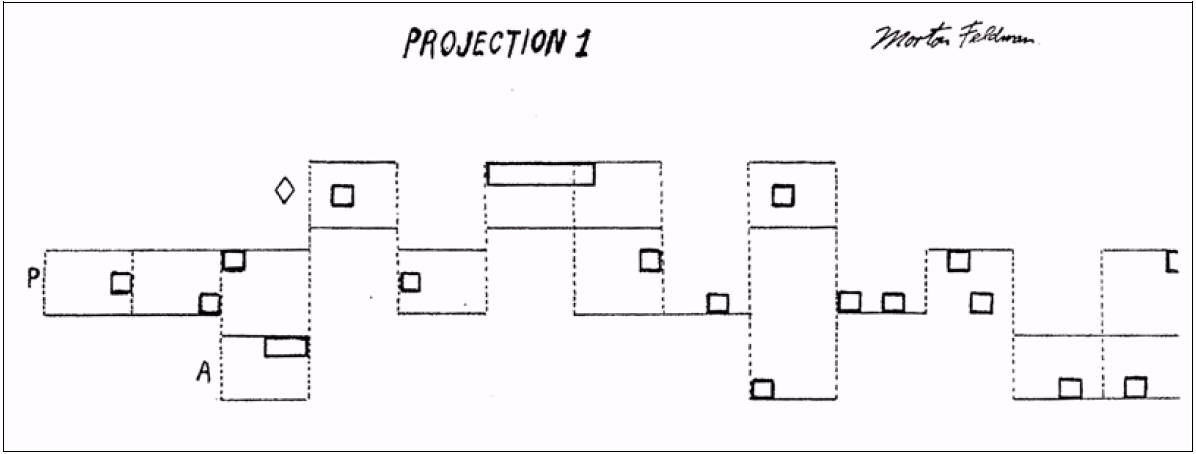
\includegraphics[width=\textwidth]{gfx/notation/MortonFeldman-Projection1.png}
	\caption[La partition de \textit{Projection 1} de Morton Feldman]{La partition de \textit{Projection 1} (1950) de Morton Feldman est une des premières partitions graphiques, caractéristique du mouvement Fluxus naissant. ©1962 C.F. Peters Corporation, avec leur aimable autorisation.}
	\label{fig:notation:feldman}
\end{figure}
\index[people]{feldman@Feldman, Morton!projection@\textit{Projection 1}}
%-------------------------- Figure : Morton Feldman ----------------------------------
\indent Les ``partitions graphiques'', c'est-à-dire recourant à l'utilisation de signes graphiques autres que les symboles habituels de la notation conventionnelle des notes sur une portée, se multiplient ainsi au milieu du \siecle{20}~siècle, et reflètent cette évolution musicale pour laquelle la notation traditionnelle s'avère insuffisante. Pour des raisons qui peuvent sembler opposées, la partition graphique a contribué à repousser à la fois les limites de ce qu'il était possible de ``fixer'' dans une composition, en la spécifiant intégralement sur un système de synthèse, et les limites de ce qu'il était concevable de laisser sujet à variations, c'est-à-dire la part confiée à l'interprétation du musicien. Les partitions de \textit{Mycènes Alpha}\index[people]{xenakis@Xénakis, Iannis!mycenealpha@\textit{Mycènes Alpha}} de Iannis Xenakis et de \textit{December 1952} de Earle Brown \index[people]{brown@Brown, Earle!december1952@\textit{December 1952}} soulignent ces deux directions (cf. Figure \ref{fig:notation:brown-xenakis}).
%-------------------------- Figure : Brown-Xenakis ----------------------------------
\begin{figure}[!htbp]
	\captionsetup{format=plain}
	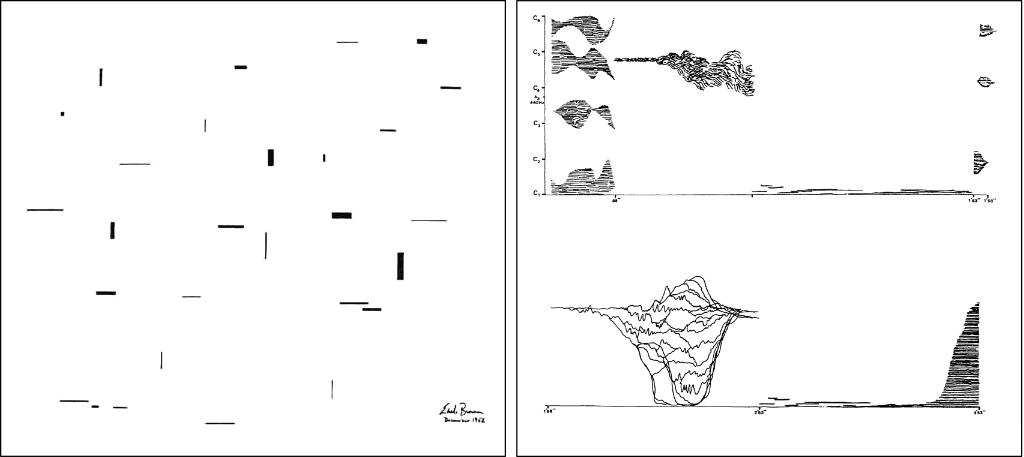
\includegraphics[width=\textwidth]{gfx/notation/Brown-Xenakis-Paysage.png}
	\caption[Partitions de \textit{December 1952} et \textit{Mycènes Alpha} (extraits)]{Extraits des partitions de \textit{December 1952} de Earle Brown (à gauche) et \textit{Mycènes Alpha} de Iannis Xénakis (à droite).}
	\label{fig:notation:brown-xenakis}
\end{figure}

\noindent Cette opposition apparente entre une œuvre totalement figée et une œuvre totalement sujette à la sensibilité des interprètes semble plutôt le résultat d'approches complémentaires visant à explorer les nouveaux domaines sonores et musicaux, tant dans leurs manifestations que dans leurs potentialités, réifiées ou fantasmées.

%-------------------------------------------------------------------------
\subsection{Œuvres ouvertes, intension, comprovisation}

%\todo{mettre un renvoi de  \ref{sec:ephemeral:longevity_stability:dynamic_scores} vers cette partie}
\noindent Parallèlement à cette part laissée à la sensibilité de l'interprète, le \textit{déroulement} de l'œuvre est devenu également sujet à variations. Si les partitions classiques se présentent généralement de manière linéaire et chronologique, les œuvres dites ``ouvertes'' fournissent aux musiciens des ``règles du jeu'' plutôt qu'une image résultant du jeu de ces règles\footnote{... d'après la définition qu'Umberto Eco en donne dans son essai ``L'œuvre ouverte'' \cite{eco_loeuvre_2015}}.\\
\indent L'œuvre ouverte peut intégrer des processus génératifs dont les résultats varient à chaque performance et la partition devient un moyen de ``noter l'imprévisible'' \cite{rebelo_notating_2010}. Jean-Louis Giavitto, dans \cite{giavitto_du_2014}, nomme ces deux types de partitions ``intensionnelles'' et ``extensionnelles'' en référence à la formulation d'ensembles en mathématique: soit ``extensive'', c'est-à-dire définie par la liste explicite des valeurs de cet ensemble, soit ``intensive'', c'est-à-dire en les définissant par une propriété générative.\\
\indent Dans ce continuum de possibilités entre œuvre fixe et improvisation libre, que Richard Dudas nomme \iquote{comprovisation} dans \cite{dudas_comprovisation:_2010}, différentes ``perspectives notationnelles''\footnote{J'emprunte ici cette expression à Sandeep Bhagwati \cite{bhagwati_notational_2013}.} peuvent être envisagées. Les différentes finalités de la représentation musicale jusqu'alors intégrées dans la partition traditionnelle gagnent en indépendance et prennent une importance variable, s'adaptant aux contextes de l'œuvre musicale et de l'interprétation. Elle peut ainsi se retrouver fragmentée en éléments qui deviennent le support d'improvisations dirigées, comme dans le \textit{Soundpainting}\footnote{Le soundpainting est un langage gestuel de direction d'improvisation multidisciplinaire, élaboré par Walter Thompson\index[people]{thompson@Thompson, Walter} dans les années 1970.} ou dans la composition \textit{Cobra}\footnote{\textit{Cobra}(1984) est une œuvre dont la composition repose sur un ensemble de signes notés sur des cartes et de règles associées, prescrivant des actions aux musiciens. Le nombre de musiciens, l'instrumentation et la longueur de la pièce sont indéterminés.} de John Zorn\index[people]{zorn@Zorn, John!cobra@\textit{Cobra}}.\\
\indent La partition définit le terrain de jeu, qui n'est pas nécessairement linéaire et qui, notamment grâce à la possibilité de produire des images animées en temps réel, peut se reconfigurer dynamiquement durant le temps de la performance.

%-----------------------------------------------------------------------------
\subsection{Partitions animées sur écran}

\noindent La disponibilité croissante des appareils numériques a conduit au développement d'un certain nombre d'applications destinées à la création de partitions à l'écran. Comme le note Lindsay Vickery dans \cite{vickery_limitations_2014} : \iquote{Ces développements suggèrent une tendance, en particulier chez les jeunes compositeurs dont la pratique s'est développée exclusivement sur ordinateur, de passer logiquement à l'étape de présenter des matériaux notationnels à l'écran.}\\
\indent Cat Hope résume les principales caractéristiques offertes par ce nouveau média dans les termes suivants \cite{hope_screen_2011}: \textit{les capacités de défilement, de permutation, de transformation, de génération et de mise en réseau du support numérique}.\\
\indent L'utilisation de l'infographie pour la représentation musicale semble être un médium de choix pour enrichir les possibilités d'écriture de partitions graphiques. En particulier, la fluidité d'adaptation du support virtuel permet d'envisager de multiples ``vues'' d'une même partition selon les contextes auxquels elle est destinée. Ainsi, la composition, la performance ou l'analyse d'une même œuvre musicale ne nécessitent pas nécessairement les mêmes représentations\footnote{Le projet ``GesTCom'' \cite{antoniadis_gesture_2014} est un exemple éloquent de l'intérêt de multiples représentations pour la composition, l'analyse et la performance. Voir par exemple : \url{https://youtu.be/KV9nQUhhyuI}}. En termes d'interprétation musicale, on peut ajouter une distinction entre l'interprétation d'une partition par un humain et une machine, ces deux types d'\textit{interprètes}\footnote{En informatique, on appelle ``interprète'' un outil ayant pour tâche d'analyser, de traduire et d'exécuter les programmes écrits dans un langage informatique.} ayant des capacités relativement différentes.\\
\indent De la même manière que les technologies numériques ont atomisé l'instrument de musique en découplant ses différentes composantes (contrôleur gestuel, cartographie, synthèse, etc. devenant modulaire), elles ont également atomisé la partition en ses différentes fonctions, de support pour la composition, la performance ou l'analyse. Il est alors nécessaire de préciser quel cas d'utilisation est en jeu et Cat Hope définit à cet effet le terme ``partition sur écran'' (\textit{screen-score}) \cite{hope_screen_2011} comme le médium présenté aux musiciens pour une performance: \iquote{Les partitions sur écran sont des compositions musicales écrites, conçues pour être interprétées ; elles ne doivent pas être confondues avec des représentations visuelles de la musique ou l'interprétation musicale des arts visuels.}\\
\indent Le concept de ``partition sur écran'' a été étudié par plusieurs chercheurs, compositeurs et musicologues (voir Winkler \cite{winkler_real-time_2004}, Clay \cite{adams_inventing_2008} ou Lee \cite{lee_real-time_2012}), qui ont discuté des avantages et des inconvénients de l'utilisation des technologies numériques pour la représentation musicale, tant dans ses aspects techniques que dans ses conséquences musicologiques. Lindsay Vickery propose par exemple une revue très détaillée dans \cite{vickery_limitations_2014}, des latences critiques permettant à un instrumentiste de lire en temps réel le matériel musical affiché et donne des conseils sur ce à quoi le compositeur doit faire attention lorsqu'il compose avec ce support.\\
\indent Ces études offrent des descriptions pertinentes et précieuses pour le compositeur qui souhaite réaliser des partitions sur écran. Cependant, il semble qu'elles puissent être complétées par une approche de la partition différente de celles envisagées dans la plupart de la littérature sur le sujet, où le point de vue est souvent celui du compositeur. La conception d'un système de partition à écran est donc polarisée par l'importance centrale de la partition, elle-même considérée comme une condition préalable à l'exécution musicale, situation qui reflète également une forte tradition de la musique classique occidentale\footnote{Une exception notable est la contribution de Georg Hajdu \cite{hajdu_disposable_2016} qui propose le concept de ``musique jetable'' pour qualifier les formes musicales \iquote{qui reposent dans une moindre mesure sur des partitions entièrement notées, telles que la ``comprovisation'' ou la performance sur laptop}\footnote{\iquote{that rely on a lesser degree on fully notated scores, such as ``comprovisation'' or laptop performance}}. Cependant, même lorsqu'elle est ``jetable'', la partition occupe ici encore une position préalable à la performance et sur laquelle l'attention reste focalisée, à la différence de l'approche proposée dans le logiciel ``John''.}. Je présenterai plus loin une ``perspective notationelle'' différente, née de la pratique instrumentale dans un contexte d'improvisation libre électroacoustique.

%---------------------------------------------------------------------

\subsection{La notation comme instrument performatif}
%TODO : nettoyer cette partie\\
%\noindent L'écriture musicale sur ordinateur est médiatisé par la machine qui interprète le code pour produire des artéfacts sonores ou visuels.
\noindent Les différents aspects précédemment cités, combinés à la nature générative des algorithmes exécutés sur ordinateurs, mettent à disposition de nouveaux outils pour l'écriture musicale, qui bouleversent la chaîne traditionnelle faisant se succéder composition, gravure, déchiffrage et interprétation d'une œuvre écrite, en abolissant une partie des délais techniques intermédiaires à ces différentes étapes. Outre l'évacuation de cette inertie dans la traduction sonore de l'écriture musicale\footnote{D'autres inerties inhérentes à l'usage des \glspl{DMI} existent cependant; le temps moyen mis par un instrumentiste ``acoustique'' comparativement à un instrumentiste ``numérique'' pour s'installer sur scène en est un exemple significatif.}, la puissance de l'écriture algorithmique réside notamment dans sa capacité à générer des motifs arbitrairement grands (potentiellement infinis) à partir d'une écriture très compacte\footnote{Toute la scène ``demo'' (\textit{demoscene}), parfois nommée \textit{bytebeat} en ce qui concerne la musique est orientée par cette recherche de ``générativité maximale'' de codes compacts. Le projet \textit{sc140tweets} qui consiste à créer une pièce musicale à partir d'un code de 140 caractères maximum --~ soit la taille d'un message sur Tweeter~-- en est une démonstration éloquente dans le domaine musical: \url{https://twitter.com/sc140tweets}. Voir également \cite{heikkila_discovering_2011}}.\\
% \begin{wrapfigure}{R}{0.5\textwidth}
% 	\captionsetup{format =plain}%
%  	\begin{center}
%     	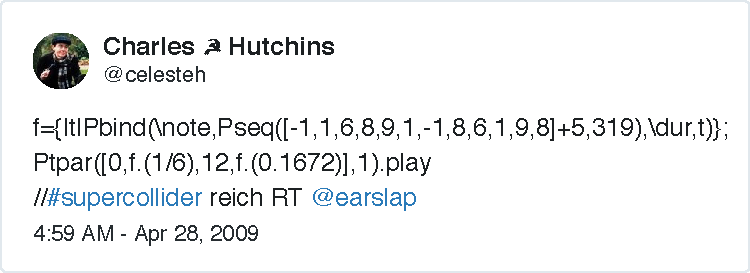
\includegraphics[width=0.48\textwidth]{gfx/notation/SC140-Reich.pdf}
%  	\end{center}
%  	\caption[\textit{Piano Phase} de Steve Reich en 140 caractères]{\textit{Piano Phase} de Steve Reich en moins de 140 caractères, tel que posté sur Tweeter pour le projet SC140 \url{https://twitter.com/celesteh/status/1635527625}.}
% 	\label{fig:notation:sc140}
% \end{wrapfigure}
\indent Ces deux aspects combinés, immédiateté de résultat et générativité, ont favorisé l'émergence de diverses pratiques s'apparentant à une forme de composition performative, c'est-à-dire, pour faire écho au début de cette section, d'une composition dans le présent de la performance. Cette composition ``performative'' peut prendre la forme d'une notation musicale en temps-réel, telle que la définissaient Arthur Clay et Jason Freeman en préface d'une édition spéciale de la \textit{Contemporary Music Review} dédiée à cette thématique \cite{clay_preface_2010}: \iquote{Nous considérons la notation musicale en temps-réel comme étant toute notation, qu'elle soit traditionnelle ou graphique, créée ou transformée durant le cours d'une performance musicale.}\footnote{We consider real-time music notation to be any notation, either traditional or graphic, which is created or transformed during an actual musical performance.}\\
\indent Une autre forme de composition en temps-réel est à l'œuvre dans la pratique du \textit{live-coding}, qui consiste à écrire en direct, sur scène, du code interprété directement par la machine\footnote{L'ouvrage collectif \cite{mclean_oxford_2018} en donne une vision riche et récente, voir sinon les contributions de Blackwell et Collins \cite{blackwell_programming_2005} ou Magnusson \cite{magnusson_algorithms_2011}.}. L'interprète est dans ce cas, le plus souvent, l'ordinateur qui génère le son à partir de ces instructions.\\
\indent Par ailleurs, l'agencement de structures musicales ``hors temps'' de la performance, dans ce que l'on nomme couramment un ``séquenceur'', et qui s'apparentait à ses origines à une simple notation symbolique d'événements musicaux selon une grille temporelle relativement fixe a considérablement évolué. L'étude du temps musical et sa modélisation mathématique a depuis permis d'assouplir ces paradigmes et de manipuler le temps de manière beaucoup plus plastique et élastique, en modélisant les relations entre événements sous formes relatives\footnote{En particulier, les relations d'Allen et le principe de tuilage \cite{berthaut_libtuile_2013} dont le modèle est à la base d'une série de séquenceurs avancés, développés au \gls{LaBRI} ces 20 dernières années, de Boxes à \textit{i-Berlioz} \cite{miranda_i-berlioz:_2019}, en passant par \textit{I-Score} \cite{desainte-catherine_interactive_2005} et \textit{OSSIA} \cite{celerier_ossia:_2015}}, son avancement par des modèles statistiques\footnote{Notamment les chaînes de Markov, utilisées depuis de nombreux systèmes de suivi de partition, comme ceux développés à l'\gls{IRCAM} depuis les années 1990.}, ou re-programmation, comme c'est le cas dans le live-coding ou dans un logiciel comme Antescofo\footnote{Cf. supra note de bas de page \ref{fn:interface:antescofo}}.\\
\indent D'autres formes apparentées ou hybrides existent, telle que la ``notation musicale animée''\footnote{Voir en particulier les travaux de Ryan Ross Smith \cite{smith_atomic_2015} dans ce domaine et son blog \url{http://animatednotation.com} sur lequel il recense les œuvres adoptant cette approche.} ou les partitions interactives dans lesquelles le contenu évolue en fonction d'interactions avec les interprètes ou le public. Un environnement de programmation comme INScore \cite{fober_inscore-environment_2012}, développé par Dominique Fober au \gls{GRAME}, est précisément conçu dans la perspective de pouvoir articuler une écriture graphique destinée à la musique de manière dynamique, non-linéaire et pluri-directionnelle, en considérant tous les objets graphiques à la fois comme des supports de représentation, des éléments de contrôles et des agents susceptibles d'être animés.\\
%\noindent L'agencement de structures musicales ``hors temps'' de la performance, qui s'est développé à la suite de l'invention de la notation musicale au Moyen Âge, est ainsi (re)devenu devenu une pratique performative dans le présent de la performance.
%(alt : Si dans ses origines, la notation musicale se sépare de l'instantanéité de la performance dans des projections vers le passé et le futur, les différentes formes d'écritures qui ont émergé depuis la seconde moitié du \siecle{20}~siècle renouent ainsi avec une pratique performative, en intégrant notamment des matériaux musicaux qui contiennent intrinsèquement leur propre temporalité.)

%Différentes perspectives sont encore à différencier dans le live-coding entre des approches basées sur un système temporel cyclique\footnote{Comme par exemple dans le logiciel \textit{TidalCycles} développé par Alex McLean}, ou plus linéaire\footnote{}.

%%%%%%%%%%%%%%%%%%%%%%%%%%%%%%%%%%%%%%%%%%%%%%%%%%%%%%%%
%%%%%%%%%%%%%%%%%%%%%%%%%%%%%%%%%%%%%%%%%%%%%%%%%%%%%%%%
%%%%%%%%%%%%%%%%%%%%%%%%%%%%%%%%%%%%%%%%%%%%%%%%%%%%%%%%
%%%%%%%%%%%%%%%%%%%%%%%%%%%%%%%%%%%%%%%%%%%%%%%%%%%%%%%%
%%%%%%%%%%%%%%%%%%%%%%%%%%%%%%%%%%%%%%%%%%%%%%%%%%%%%%%%
\section{John, un instrument pour la comprovisation}

\subsection{Genèse d'une notation}

\noindent Dans le cas des performances de ONE (Figure \ref{fig:notation:one-fullband}), qui sont basées sur une pratique d'improvisation libre sans composition préalable, la focale est déplacée du côté de l'instrumentiste. L'élément central n'est pas la partition, mais l'écoute et la compréhension du son et des autres musiciens. La partition (s'il est encore possible de l'appeler ainsi) émerge souvent après les séances d'improvisation et sa présence ne doit pas se faire au détriment de l'attention mutuelle. Dans cette perspective, il est possible d'envisager que le musicien adapte lui-même la représentation musicale à ses propres besoins, en fonction des parties qu'il doit jouer, de ses préférences personnelles, des différents mouvements de la partition, etc.\\
\indent Dans le cas particulier où les instruments sont numériques et programmables, l'utilisation d'un système de partition en réseau offre également la possibilité de déléguer certains paramètres de l'instrument à un contrôle externe pris en charge par la partition. Dans une situation d'improvisation, la négociation entre ce contrôle automatisé et le choix du musicien implique une médiation que j'évoquerai dans la section \ref{sec:notation:score_for_humans_and_machines}.

\subsubsection{Présentation de ONE}
\index[people]{one@ONE (Orchestre National Électroacoustique)}
\noindent Les sept musiciens de l'ensemble ONE (cf. figure \ref{fig:notation:one-fullband}) sont tous profondément impliqués dans le domaine de l'informatique musicale avec des spécialités diverses dans les domaines de la pratique instrumentale, de la composition, de la facture instrumentale, de la recherche en sciences musicales et de l'éducation. Nous pratiquons tous des \glspl{DMI} dont nous avons conçu le logiciel\footnote{La plupart de ces \glspl{DMI} utilisent le logiciel Max pour le design de l'interaction, voire la synthèse.} et parfois aussi l'interface hardware, dans une certaine mesure.
A l'origine de notre collaboration, il n'y avait pas d'autre projet que celui de tenter l'expérience de jouer une ``musique de sons'' avec cet \textit{instrumentarium} numérique hétéroclite, sans grille, sans théorie musicale, sans accord préalable sur la forme et le contenu\footnote{Des extraits video de ONE en concert sont disponibles ici: \url{https://youtu.be/lBVNwGeTxFA}}.
%-------------------------- Figure : ONE ----------------------------------
\begin{figure}[!htbp]
	\captionsetup{format=plain}%
	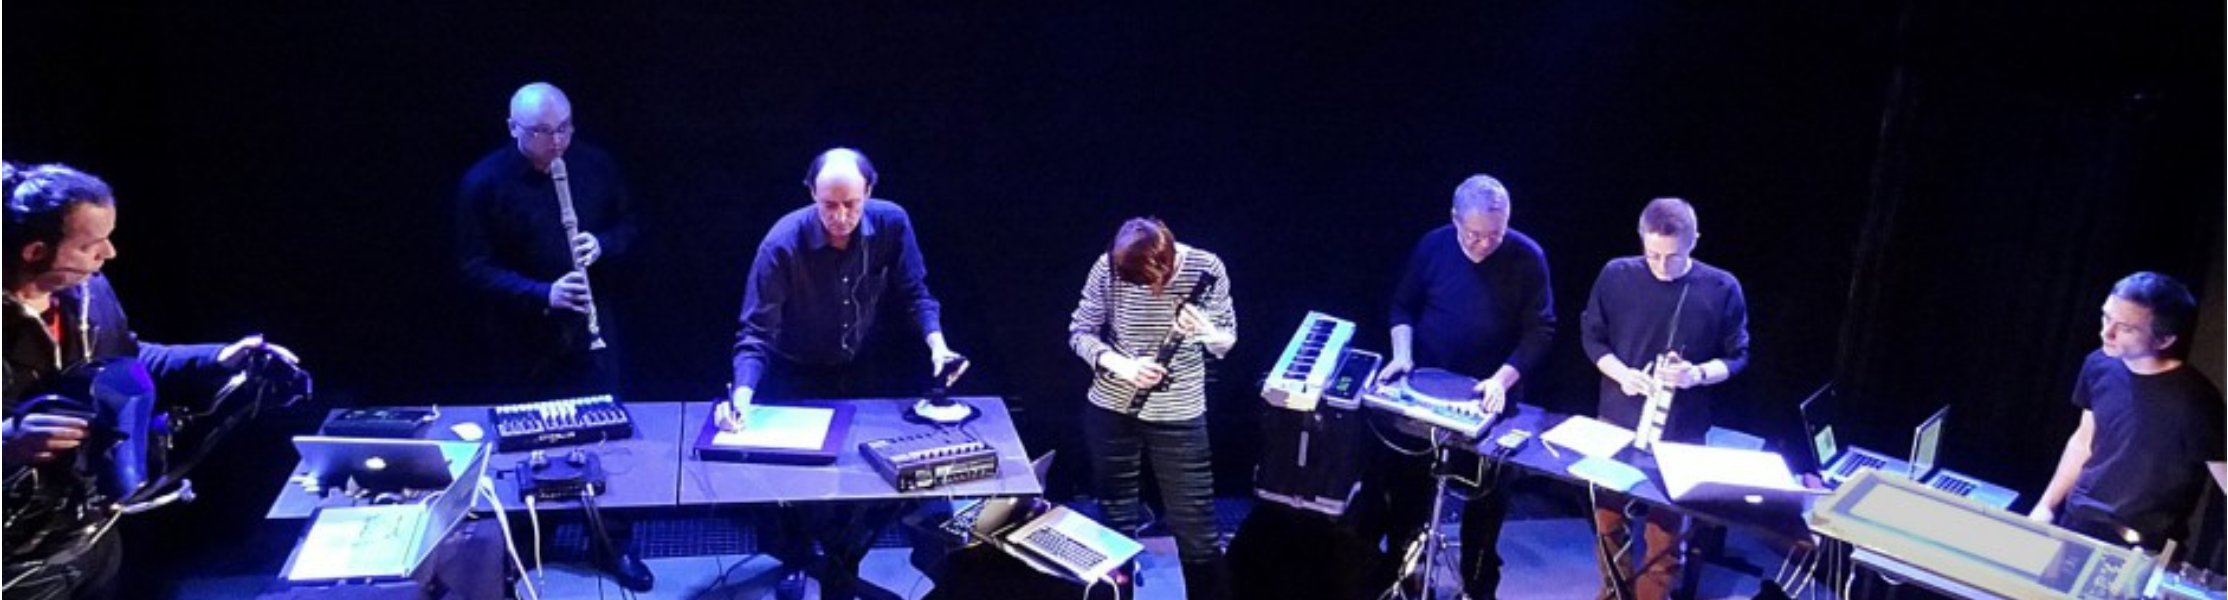
\includegraphics[width=\textwidth]{gfx/notation/ONE-fullBand.png}
	\caption[Les membres de ONE et leurs DMIs]{Les membre de ONE sur scène avec leurs \glspl{DMI}. De gauche à droite : Serge de Laubier au Méta-Instrument 3, Pierre Couprie à la flûte augmentée et interfaces MIDI, Hugues Genevois au Calliphone, Laurence Bouckaert au Karlax, György Kurtág Jr. au Handsonic, Jean Haury au Méta-Piano, Vincent Goudard au Filigramophone.}
	\label{fig:notation:one-fullband}
\end{figure}
%-------------------------- Figure : ONE ----------------------------------
\index[people]{delaubier@De Laubier, Serge!ONE@\textit{ONE}}
\index[people]{couprie@Couprie, Pierre!ONE@\textit{ONE}}
\index[people]{genevois@Genevois, Hugues!ONE@\textit{ONE}}
\index[people]{bouckaert@Bouckaert, Laurence!ONE@\textit{ONE}}
\index[people]{kurtagjr@Kurtág, György, Jr.!ONE@\textit{ONE}}
\index[people]{haury@Haury, Jean!ONE@\textit{ONE}}
\index[people]{goudard@Goudard, Vincent!ONE@\textit{ONE}}

\subsubsection{Improvisation libre et expérimentation}

\noindent Plusieurs séances d'improvisation ont été l'opportunité de découvrir nos sons, nos styles de jeu, notre vocabulaire musical. Ces moments de répétition ont été avant tout l'occasion de performances anarchiques, guidées uniquement par le fil de notre écoute, de confrontation, de mélange, de collision, de superposition d'objets et d'espaces sonores, ainsi que de moments de discussion et de réglages de nos dispositifs de jeu.\\
\indent Ces sessions ont également fait l'objet d'exercices d'improvisation classiques : recherche de fusion timbrale et de contrepoints, passages fugués entre musiciens, accompagnement d'un soliste, travail sur les nuances pianissimo, ou improvisation ``dans le style'' d'une pièce connue. Finalement, les enregistrements audio nous ont permis de ré-écouter les improvisations parfois longues et ininterrompues pour en extraire des idées musicales intéressantes.\\

\subsubsection{Structurer le temps}

\noindent La question de la structure globale d'un concert en mouvements musicaux est apparue durant la préparation de la première performance en public de ONE. L'absence d'une partition structurant la durée du concert nous a conduits à suivre un scénario narratif inspiré d'un roman de Jules Verne. Ainsi, le concert consistait en une série de chapitres, simplement identifiés par des intertitres tenant lieu de paysages sonores exotiques et imaginaires à explorer.\\
\indent Peu à peu, ces expériences ont donné lieu à l'émergence d'un vocabulaire musical plus atomique, représentant des atmosphères et des mouvements définis collectivement, que nous avons appelés ``karmas''\footnote{La relation avec ce concept indien est lointaine, mais elle comporte un sens séduisant qui fait écho à la façon dont nous les voyons dans la performance : l'ensemble des actions représentées par le karma influence l'avenir de l'individu. De même que l'interprétation musicale d'un \textit{karma} (tel que nous le définissons) est soumise aux actions des musiciens et tout accident, la bifurcation par rapport à la partition prévaudra sur l'évolution musicale plus que la partition elle-même.}. Les différents moments de jeu et de discussion nous ont amenés au développement d'autres objets conceptuels qui ont été en partie réalisés sous la forme d'un logiciel surnommé ``John, le semi-conducteur''\footnote{En anglais ``John, the semi-conductor'', ``conductor'' signifiant chef d'orchestre, ce subtil jeu de mot se perdant malheureusement dans sa traduction française...}.\\
\indent L'origine du développement de John est ainsi liée au désir de trouver un moyen de structurer le temps musical en différents mouvements dans la perspective de concerts librement improvisés d'une durée assez longue. 

\subsubsection{Stimuler la pratique en l'absence de chef}
%
\noindent Une autre motivation résidait dans la possibilité de générer des improvisations variées, afin de ne pas toujours répéter les mêmes textures et structures formelles telles que des séquences de cycles ascendants-descendants.\\
\indent De plus, nous cherchions des moyens de stimuler l'exploration de combinaisons et d'idées musicales inhabituelles qui nous poussent hors de notre zone de confort. La proposition de diviser mathématiquement le temps en séquences pour permettre à tous les ensembles possibles (solo, duo, trio, ... jusqu'au tutti), a été la première impulsion pour le développement d'un générateur de partition capable de produire automatiquement de telles distributions.\\
\indent Comme les opinions divergeaient au sein du groupe sur l'équilibre entre règles et absence de règles, un principe clé a permis de trouver un terrain d'entente : John est un ``semi-conducteur'', un ``sous-chef d'orchestre''. Cela signifie que les partitions créées avec John ne sont qu'une proposition, que chaque membre du groupe est libre de suivre ou non, selon le contexte musical qui ne prend véritablement forme qu'au moment même de la performance. L'écoute reste donc la règle essentielle du jeu, l'emportant sur un suivi aveugle de la partition. En particulier, sont laissées à l'appréciation de chaque musicien l'articulation entre les différentes parties de la partition, qu'elles soient tuilées ou disjointes, ou encore la décision de jouer quand il n'est pas censé le faire (ou inversement), etc.\\
\indent Ce principe a pour conséquence directe une épuration dans le design visuel de la partition, dont le but est de permettre à chaque musicien de se situer en un coup d'œil dans la partition, sans monopoliser son attention au détriment des autres musiciens et du son. Le but est donc très différent de celui poursuivi dans d'autres systèmes de notation musicale sur écran, comme ceux explorés dans des travaux impliquant du déchiffrage en direct de partition dynamique \cite{freeman_extreme_2008}.\\
\indent Ainsi, John permet la gestion collective du temps, que ce soit lors des répétitions, de la composition ou des performances, en fournissant un support de représentation partagé. Une brève description du logiciel pour en saisir les grandes lignes précédera une discussion sur les différents aspects liés à cette gestion de groupe.

%%%%%%%%%%%%%%%%%%%%%%%%%%%%%%%%%%%%%%%%%
\subsection{Description technique}

\noindent John s'appuie sur une architecture client / serveur, dans laquelle chaque musicien visualise une interface client dans un navigateur web, sur laquelle il peut agir. Cette interface se compose de deux parties, un générateur de partition d'une part et une visualisation interactive de la partition d'autre part.
%-------------- Figure : John client interface -------------
\begin{figure}[!htbp]
	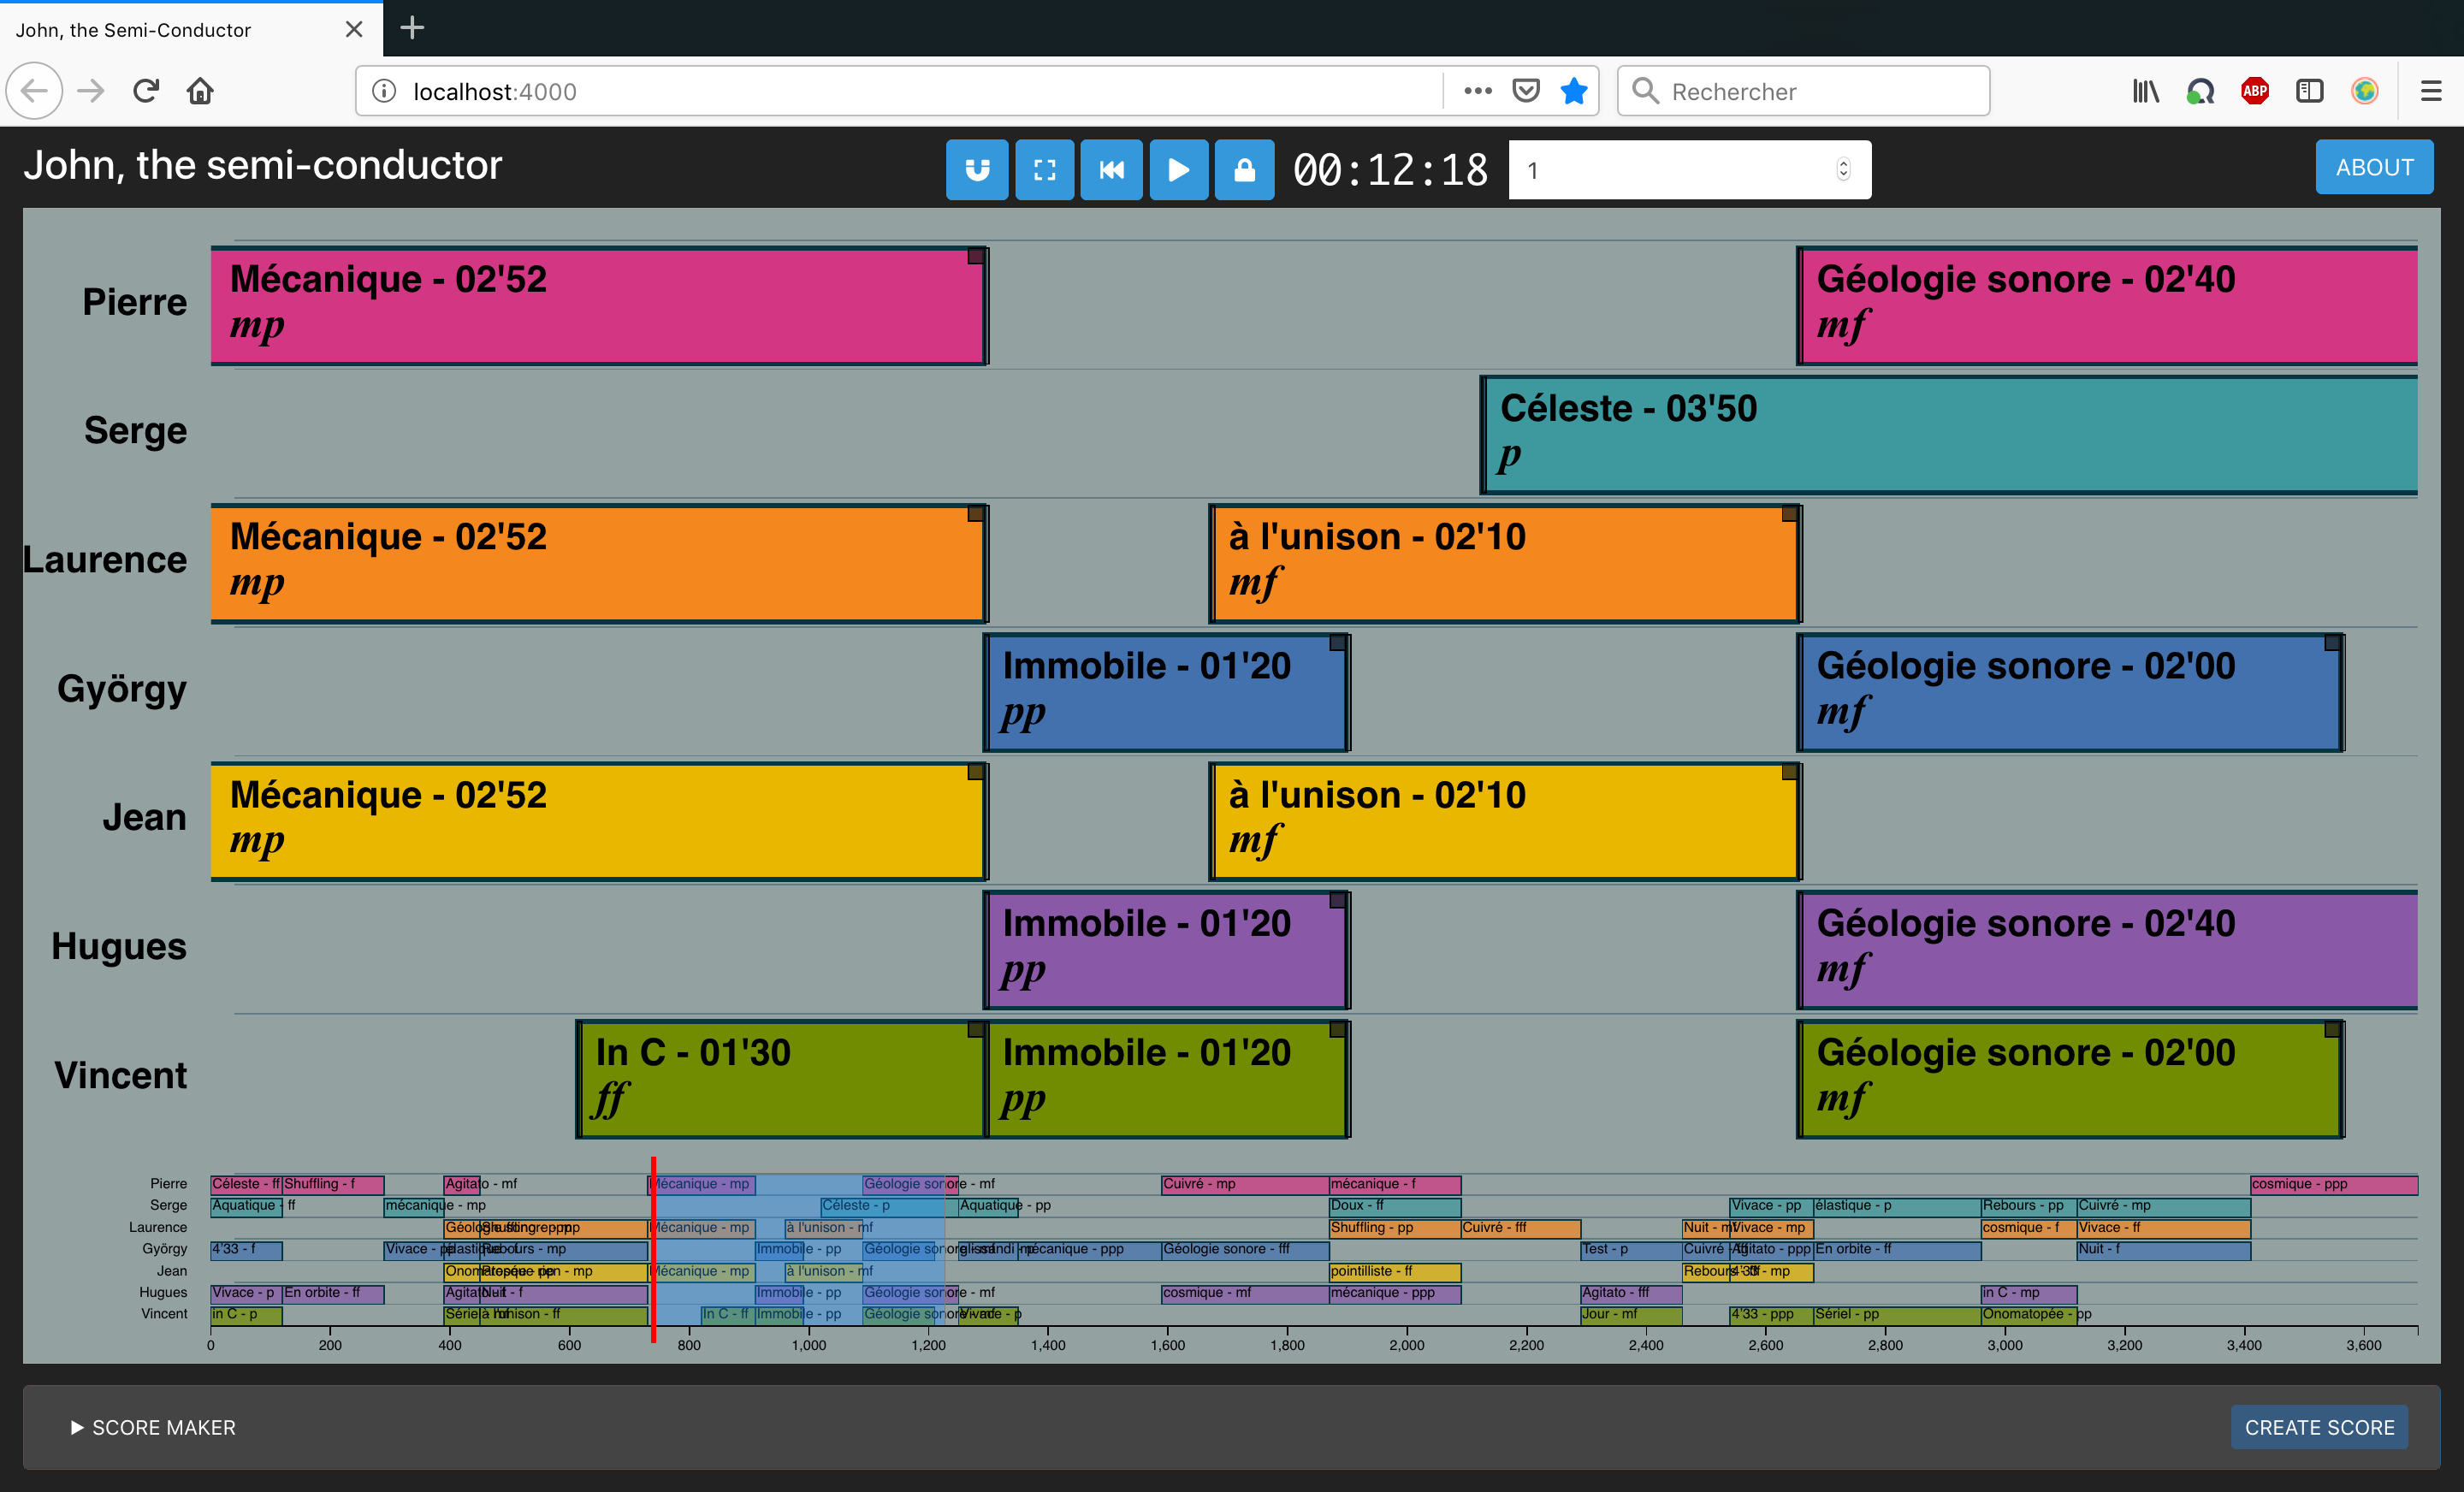
\includegraphics[width=\textwidth]{gfx/notation/John-snapshot.png}
	\caption[John : capture écran de l'interface client]{Aperçu de l'interface de John tournant dans un navigateur web.}
	\label{fig:notation:john-snapshot}
\end{figure}
%-------------- Figure : John client interface -------------
\subsubsection{Générateur de partitions}

\noindent Le générateur de partitions permet de créer très rapidement des propositions musicales en ne spécifiant que des contraintes globales :
\vspace{-1em}
\begin{itemize}[noitemsep]
	\item la durée globale de la partition;
	\item le nombre minimal et maximal de joueurs;
	\item la durée minimale et maximale des blocs;
	\item une liste de \textit{karmas} identifiant une ambiance musicale particulière, selon un vocabulaire défini en commun durant les séances d'improvisation;
	\item une liste de nuances de \textit{pianississimo} à \textit{fortississimo}.
\end{itemize}
%
\noindent Une fois ces contraintes spécifiées, le générateur de partition produit une proposition aléatoire respectant ces conditions, composée d'une séquence de blocs temporels associant un karma et une nuance. Cette proposition peut ensuite être ajustée dans l'interface d'édition / visualisation.

%----------------------------------------------------------------------------------------------------------
\subsubsection{Visualisation interactive}

\noindent Cette interface représente des blocs disposés sur une abscisse chronologique. Elle se compose d'une \textit{vue globale} réduite d'une part, offrant une vue d'ensemble partagée de la partition dans son intégralité, et d'une \textit{vue locale} zoomable, située au-dessus de la \textit{vue globale}. Sur la \textit{vue globale} se trouve une tête de lecture commune et synchrone à tous les clients, ainsi qu'un empan temporel (en rouge et bleu, respectivement, sur la figure \ref{fig:notation:john-snapshot}) définissant la durée affichée sur la \textit{vue locale}. Cet empan est défini individuellement par chaque musicien sur son client web et varie généralement d'une dizaine de secondes à quelques minutes selon la granularité temporelle de la partition et la préférence de chacun.\\
\indent Tous les paramètres de contrôles sont accessibles dans l'ensemble des clients, permettant à chacun d'éditer la partition : générer une nouvelle instance, déplacer et modifier la durée des blocs et leur contenu (\textit{karma} et \textit{nuance}), démarrer la lecture, modifier la vitesse de lecture, déplacer la tête de lecture pour démarrer à un moment donné de la partition. Ces changements sont immédiatement appliqués à l'ensemble des autres clients de John.\\
\indent L'utilisateur peut également définir des paramètres locaux qui n'affecteront que son interface client : la visibilité des différentes pistes, la durée de sa \textit{vue locale} et la synchronisation (ou non) de sa vue locale au curseur de lecture, à l'aide du bouton ``link'' (en forme de cadenas sur la figure \ref{fig:notation:john-snapshot}).

%----------------------------------------------------------------------------------------------------------
\subsubsection{Implémentation}

\noindent Après une première version développée en Max\footnote{\url{https://cycling74.com}}, l'application a été portée en \gls{HTML5} réactif à l'aide de l'environnement Meteor\footnote{\url{http://meteor.com}}. Ceci permet l'édition collective sur la plupart des plateformes (y compris les plateformes mobiles) connectées à un réseau local, via un simple navigateur web. La visualisation a été réalisée à l'aide de la bibliothèque D3.js\footnote{\url{https://d3js.org}}.\\
\indent Les partitions sont sauvegardées au format \gls{JSON} sous la forme d'une liste d'événements avec un identifiant unique, un index de piste, un temps de début, une durée et un certain nombre de propriétés telles que le karma et les nuances. Pendant la lecture, le temps et les événements de la partition sont envoyés par \gls{OSC} sur le réseau et récupérables dans Max en tant que messages MP (cf. section \ref{sec:algorithms:MP}).

%%%%%%%%%%%%%%%%%%%%%%%%%%%%%%%%%%%%%%%%%
\subsection{John en pratique}
%-----------------------------------------------------
\noindent Cette section présente divers constats sur les conséquences résultant de l'usage de John dans la pratique musicale de ONE.

\subsubsection{Composition générative}

\noindent Le générateur de partitions a fait gagner beaucoup de temps pendant les répétitions, en offrant immédiatement une structure musicale possible. Aussi arbitraire que soit cette structure, sa fonction principale est de stimuler la performance musicale via sa prescription la plus minimale : \textit{quand jouer} (ou ne pas jouer). Ainsi, les propositions sont souvent testées telles quelles avant d'être ajustées collectivement en fonction de ce que les membres du groupe trouvent intéressant ou non. Il est alors possible de faire évoluer cette structure musicale, avec apparemment plus d'efficacité que si l'on ne partait de rien.

%----------------------------------------------------------
\subsubsection{Distribution de la participation}

\noindent Le fait que John propose explicitement une distribution du temps de jeu entre chaque musicien a conduit à des configurations d'ensemble que nous n'aurions pas nécessairement tentées, en particulier les ensembles réduits (solo et duo), la tentation de jouer étant parfois trop grande pour laisser s'installer ces configurations minimales, plus fragiles et d'une certaine manière, plus risquées.\\
\indent De plus, avoir des moments de pause explicites permet de mieux anticiper ses entrées. En effet, les \glspl{DMI} ont souvent une dimension ``méta-instrumentale''\footnote{C'est-à-dire qu'il peut être totalement reconfiguré pendant la représentation pour offrir un tout autre ensemble de sons, de processus et de modes de jeu.} et exposent généralement un grand nombre de paramètres, dont tous ne sont pas nécessairement accessibles directement. Ces moments de pause planifiés peuvent permettre de prévoir le temps dont dispose chaque instrumentiste pour gérer de telles reconfigurations de paramètres.

%------------------------------------------------------------
\subsubsection{Synchronisation}

\noindent Dans une situation d'improvisation libre, la synchronisation entre les musiciens est entravée par l'inexistance de règles idiomatiques. En particulier, l'absence de pulsation et de mesure rend cette synchronisation plus difficile encore quand le nombre de musicien augmente et prive souvent l'improvisation libre de transitions franches dans la pratique d'ensemble.\\
\indent Le chef d'orchestre, lorsqu'il y en a un, fournit des repères temporels précis, par la battue et d'éventuelles indications pour le jeu. Outre les problèmes liés à la hiérarchie des relations, posés par le rôle d'un leader dans un groupe d'improvisation, et analysées par Clément Canonne dans \cite{canonne_improvisation_2012}, confier la direction d'une improvisation à une personne\footnote{Comme c'est le cas dans le \textit{Soundpainting} de Walter Thompson.} reste limité par le fait qu'elle ne peut agir que dans le présent, et que cela exige une attention quasi-permanente des musiciens envers le chef, au détriment de celle qu'ils peuvent porter à leurs pairs. En effet, le chef d'orchestre est essentiellement dans un rapport d'immédiateté avec les musiciens, qui ne peuvent guère savoir quand aura lieu le prochain événement. À cet égard, la représentation offerte par John condense d'une certaine manière la partition et le chef d'orchestre en un seul et même support visuel. Cette partition animée offre en effet des repères visuels qui indiquent la simultanéité de plusieurs événements musicaux, et son défilement sous la tête de lecture, accompagné de compte-à-rebours individuels, permet une synchronisation précise entre les musiciens lors des transitions.

%----------------------------------------------------------------------------------------------------------
\subsubsection{Support visuel pour des repères musicaux}

\noindent Malgré la disponibilité d'outils d'analyse\footnote{Tels que EAnalysis \cite{couprie_eanalysis:_2016} ou l'Acousmographe du \gls{GRM} \cite{favreau_lacousmographe_2010}.} et l'existence d'un certain vocabulaire pour décrire les objets sonores et musicaux dans la musique électroacoustique\footnote{en particulier les ``objets sonores'' de Pierre Schaeffer\index[people]{Schaeffer, Pierre@} \cite{schaeffer_traite_1966}, les ``images-son'' de François Bayle\index[people]{Bayle, François@} \cite{bayle_musique_1993} ou encore les \gls{UST} du \gls{MIM} \cite{delalande_les_1996}.}, il n'existe aucune norme de notation prescriptive pour les \glspl{DMI}. L'absence d'un vocabulaire unanime, la singularité des instruments et la formidable palette sonore qu'ils offrent, ne facilitent pas l'exercice consistant à identifier et discuter ce qui vient d'être joué lors d'une longue séance d'improvisation (manquant de pouvoir parler ici de ``répétition''). Une partition minimale telle que celle proposée par John facilite cette identification et permet de retravailler des moments précis après une longue performance. La réduction que la notation symbolique opère sur le résultat sonore complexe d'une performance permet à chacun de se retrouver rapidement dans l'espace temporel d'une improvisation, plus rapidement du moins que si l'on devait se référer à l'enregistrement sonore.

%----------------------------------------------------------------------------------------------------------
\subsubsection{Une écologie de l'attention}

\noindent L'improvisation libre électroacoustique requiert une attention considérable des musiciens envers les autres musiciens, leur instrument et, de toute évidence, au son\footnote{Il n'est pas question ici de prétendre que la musique non-improvisée ne requiert pas d'attention mutuelle des musiciens, mais elle se pose toutefois en des termes légèrement différents, les éléments ``stables'' de la partition y étant par définition plus nombreux.}. À cet égard, les \gls{DMI} présentent souvent l'inconvénient supplémentaire, par rapport aux instruments acoustiques, de capter une partie de l'attention visuelle en raison de la présence fréquente d'un écran, de nombreux paramètres d'interaction et d'une interface parfois dépourvue de retours ou de repères tactiles qui permettraient d'y accéder sans avoir besoin de les regarder. De plus, les musiciens numériques préparent souvent leur instrumentarium juste avant la représentation\footnote{Thor Magnusson et Kris Kiefer nomment cette préparation de code une ``pre-grammation'' dans \cite{kiefer_live_2019}} avec un ensemble choisi d'éléments musicaux \textit{ad hoc} (lorsqu'ils ne le codent pas en direct, comme c'est le cas dans le live-coding), ce qui complique encore la connaissance ``kinesthésique'' de l'ergonomie de l'instrument, sans aucune aide visuelle.\\
\indent La conception de ``John'' a été ainsi motivée par une économie de la charge cognitive des musiciens. Pouvoir en partie personnaliser son interface de visualisation ne signifie donc pas y ajouter davantage de données visuelles, mais plutôt n'afficher que ce qui est nécessaire, au profit de l'attention mutuelle.

%----------------------------------------------------------------------------------------------------------
\subsubsection{Partitions pour humains \emph{et} machines}
\label{sec:notation:score_for_humans_and_machines}

\noindent Pendant la lecture de la partition, le serveur envoie des données au format MP\footnote{Cf. supra, section \ref{sec:algorithms:MP}} aux clients lorsque des événements commencent ou se terminent. Ces informations peuvent être utilisées par l'instrument du musicien (si toutefois son \gls{DMI} est connecté au réseau). Mais, comme John n'est qu'un ``semi-conducteur'', ses messages peuvent tout aussi bien être soumis à l'approbation du musicien/client pour permettre une certaine flexibilité dans la façon dont le musicien adhère à la partition.\\
\indent Ainsi, il est possible d'imaginer qu'un \textit{karma} spécifique rappelle un pré-réglage dans l'instrument du musicien, correspondant à l'esprit de ce \textit{karma}. Mais si le musicien est encore en train de jouer le \textit{karma} précédent, il/elle ne voudra probablement pas que cette notification change automatiquement sa configuration avant d'avoir terminé la phrase musicale en cours. Cette ``évaluation paresseuse''\footnote{J'emprunte ici ce terme utilisé dans le domaine de la programmation récursive, qui consiste à évaluer une expression uniquement quand le résultat de cette expression devient nécessaire. Dans notre cas toutefois, c'est possiblement le musicien qui décide de cette évaluation.} rend l'utilisation de John un peu différente de celle des séquenceurs traditionnels.
% TODO : rajouter une figure du patcher Max de réception des data
%----------------------------------------------------------------------------------------------------------
\subsubsection{Montrer la partition ?}

\noindent Rendre lisible les interactions entre les musiciens dans les performances d'improvisation peut contribuer à l'appréciation globale de la performance par le public. Pourtant, avec les \glspl{DMI}, le découplage spatial et énergétique entre les gestes de l'instrumentiste et la localisation de l'énergie sonore (sur un haut-parleur possiblement distant) brouille cette lecture. Les systèmes de partition sur écran offre la possibilité de partager l'affichage de la partition avec le public plus facilement que ne le permettent les partitions imprimées et peuvent ainsi aider à cette lisibilité avec le risque, cependant, qu'elle ``entrave les aspects performatifs dramatiques de l'œuvre'' parmi d'autres raisons suggérées par Cat Hope dans \cite{hope_screen_2011}.\\
\indent Bien que la partition de John n'ait jamais été montrée directement au public pour cette raison particulière, elle a été utilisée pour contrôler des effets vidéo et de lumières\footnote{Il s'agissait par exemple d'éclairer les musiciens censés jouer, de modifier la teinte de la lumière en fonction des karmas, de projeter des ondes sonores agrégées comme traces de la partition, de synchroniser des vidéos, etc.}, à la fois des raisons scénographiques et pour aider l'écoute à la compréhension de la musique.

%%%%%%%%%%%%%%%%%%%%%%%%%%%%%%%%%%%%%%%%%
\subsection{Perspectives}

\noindent Les membres de ONE ont reconnu que John aidait le processus créatif. Cependant, il reste des questions ouvertes comme la synchronisation collective sur les passages rythmiques. En particulier, anticiper un processus dynamique n'est pas une tâche triviale et nécessiterait probablement des outils spécifiques à cette fin, telles que les animations proposées par Ryan Ross Smith dans \cite{smith_atomic_2015}.\\
\indent Le concept de vues \textit{locale} et \textit{globale} pourrait probablement être généralisé à d'autres paramètres partageables. Par exemple, pouvoir démarrer une lecture locale pour s'entraîner ou préparer son instrument par soi-même. De même, il serait utile de travailler sur une autre partition que celle chargée sur les autres clients. Cette désynchronisation soulève cependant des problèmes de conflits de versionnage, dont la prise en compte dépasse pour l'instant les possibilités offertes par John.\\
\indent Le portage de John sur une technologie web a été en partie motivé par la possibilité de futurs concerts impliquant un grand nombre de musiciens et dans lesquels chaque musicien pourrait voir sa partie avec un simple navigateur web. D'autres développements seront nécessaires pour pouvoir réaliser de telles performances, qui posent là-encore des questions d'ergonomie visuelle.\\
\indent Dans l'ensemble, les partitions informatisés laissent place à de nombreuses interactions possibles pendant la durée de la performance. Leur design pourrait probablement tirer parti du fait de les considérer comme un instrument collectif, dont chaque musicien, en incluant aussi le public et son écoute active, pourrait jouer.


\section{Conclusion}

\noindent Après avoir présenté et analysé certains aspects particuliers de la notation musicale qui prennent une importance critique dans la pratique des \glspl{DMI}, j'ai retracé la naissance du logiciel John, un logiciel hybride servant d'outil collaboratif pour la création de partitions minimale, ainsi que de guide temporel durant la performance.\\
\indent Ce logiciel s'est construit très empiriquement, sur la base des éléments ayant émergé durant les sessions d'improvisation de ONE. En particulier, la notion de ``\textit{karma}'' comme unité musicale partagée\footnote{partagée sans être pour autant consensuelle, tout le monde ne rattachant pas exactement les mêmes sons, ou les mêmes idées, aux même karmas.} fait écho à ``l'entomologie musicale'' évoquée au chapitre \ref{ch:ephemeral}. Toutefois, cette notion agit de manière bidirectionnelle, car certain \textit{karmas} ont été proposés (et accepté ou rejeté par le groupe, selon les cas) sans qu'ils aient émergés de sessions d'improvisation, mais en tenant lieu de référence commune\footnote{Par exemple, le \textit{karma} ``Géologie Sonore'' fait référence à la pièce éponyme de Bernard Parmegiani\index[people]{Parmegiani@Parmegiani, Bernard!denaturasonorum@\textit{De Natura Sonorum}}}.\\
\indent À la différence de la plupart des logiciels de composition, John n'a pas été conçu selon la perspective notationelle du compositeur, pour qui la partition occupe généralement une place centrale, mais selon la perspective performative des musiciens dans un contexte de musique improvisée, exigeant une attention mutuelle particulière. Son design visuel a été adapté en conséquence pour minimiser la charge cognitive des instrumentistes. Enfin, la possibilité de venir contrôler des processus externes depuis John permet d'envisager d'autres nuances dans l'articulation possible entre œuvre fixe et œuvre improvisée




% à  qui s'est construit selon une démarche 

% \section*{extra}
% Intérêt génératif de la partition / gameification  :
% Sarah Fdili Alaoui : motate \url{http://saralaoui.com/2015/07/motate}
% the thing from the future \url{https://situationlab.org/tag/the-thing-from-the-future}

% - étape 1 : identifier les patterns \\
% - étape 2 : leur donner une entité atomique et manipulable\\
% - étape 3 : créer des nouveaux scénarios avec ces blocs